

\section{Preshower detectors}

\subsection{Central preshower detector}
%%%%%% SLIDE
\begin{frame}{\textcolor{Goldenrod}{Preshower detector }}
  \begin{overlayarea}{\textwidth}{\textheight}
    \begin{figure}[h]\centering
      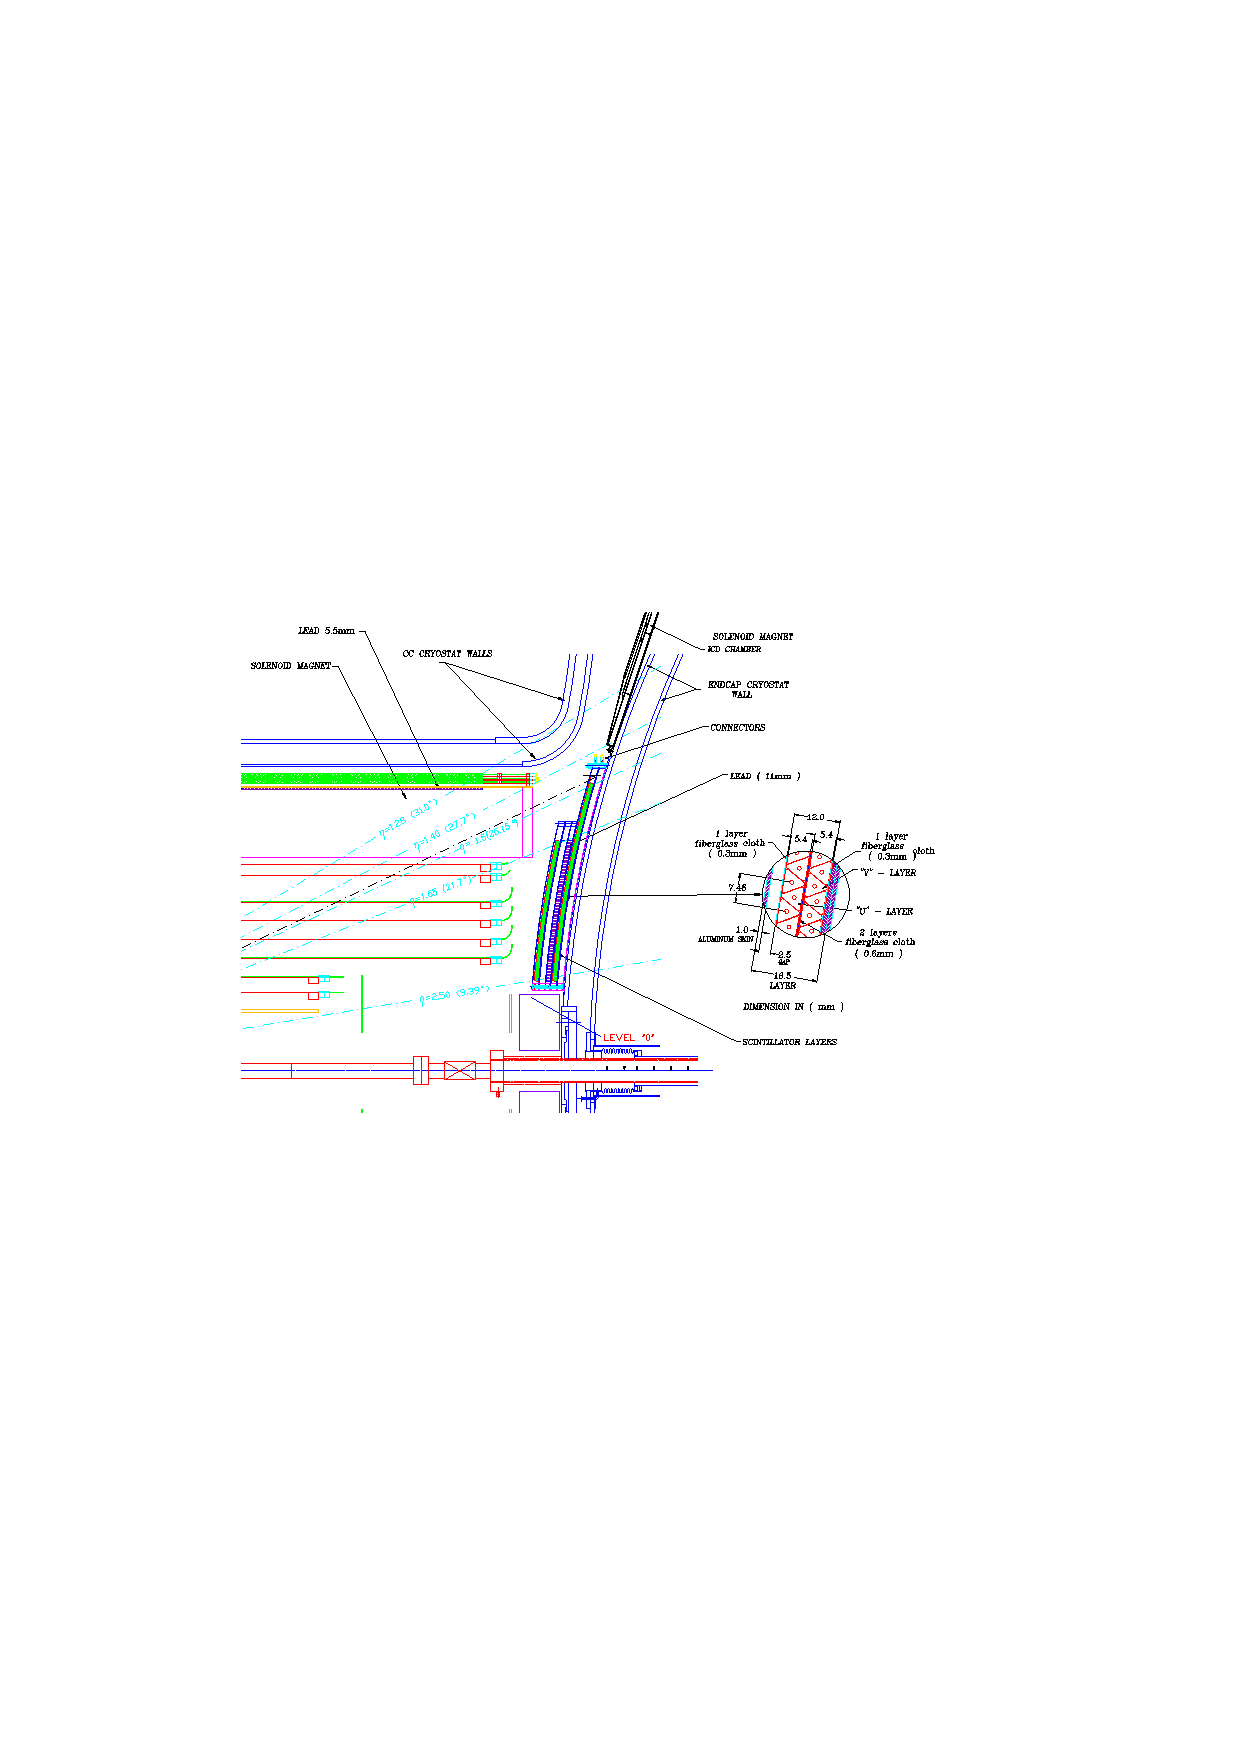
\includegraphics[height=0.55\textheight, width=0.9\textwidth]{./Images/29_PS_forward.pdf}
    \end{figure} 
    \itt
  \item \hlt{black}{calorimetery as well as tracking detectors:\\}
    \alert{electron ID and background rejection at online triggering and
      offline reconstruction.}
    \tti
  \end{overlayarea}
\end{frame}


%%%%%% SLIDE
\begin{frame}{\textcolor{Goldenrod}{Central Preshower Detector}}
  \(
  \<{0.37\textwidth}
  \img{29_PS_unit_cell.pdf}\\
  \img{30_PS_triangle_strip}\\
  \img{29_PS_central.pdf}
  \>
  \<{0.7\textwidth}
  \itt
\item[$\Box$] three concentric cylindrical layers of $1280$ scintillators,
  arranged in an axial-u-v ($23^{\circ}$) geometry
\item[\Box] scintillators:\\
  \itt
  \item \alert{triangular strips with a wavelength-shifter at
    center of each strip and a waveguide transfering light to outer
    VLPCs.}
  \item made of extruded polystyrene (PS), \it{paraterphenyl (PT) $1$\%, and
      diphenyl stilbene (DS)$0.15$\%}
    \tti
  % \item \alert{each scintillator strip is machine-wrapped in aluminized
  %   mylar for optical isolation}
  \tti
  \>
  \)
\end{frame}


\subsection{Forward preshower detector}
%%%%%% SLIDE
\begin{frame}{\textcolor{Goldenrod}{Forward Preshower detector }}
  \(
  \<{0.75\textwidth}
  \itt
  \note{The upstream layers are known as the minimum ionizing particle,
    or MIP, layers while the downstream layers behind the absorber are
    called the shower layers.}
\item[$\bullet$] Charged particles passing through the detector will register
  minimum ionizing signals in the MIP layer $\to$ tracking.
  
\item[$\bullet$] {\small \alert{Electrons shower in the absorber $\to$
      a cluster of energy, % (typically on the order of three strips wide),
      which is then matched to MIP-layer signal.}}
\item[$\bullet$] {\small Photons will not generally interact in the
    MIP layer, but will produce a shower signal in the shower layer.}
\item[$\bullet$] {\small \textcolor{blue}{Heavier charged particles
      are less likely to shower, typically producing a second MIP signal in
      the shower layer.}}
  \tti
  \>
  \<{0.4\textwidth}
  \img{30_PS}\\
  {\scriptsize FPS module with  $u-v$ MIP
    and shower layers, separated by a lead and stainless steel absorber.}
  \>
  \)
\end{frame}

%%%%%% SLIDE
\begin{frame}{\textcolor{Goldenrod}{Forward Preshower Detector}}
  \begin{overlayarea}{\textwidth}{\textheight}
    \begin{figure}[h]\centering
      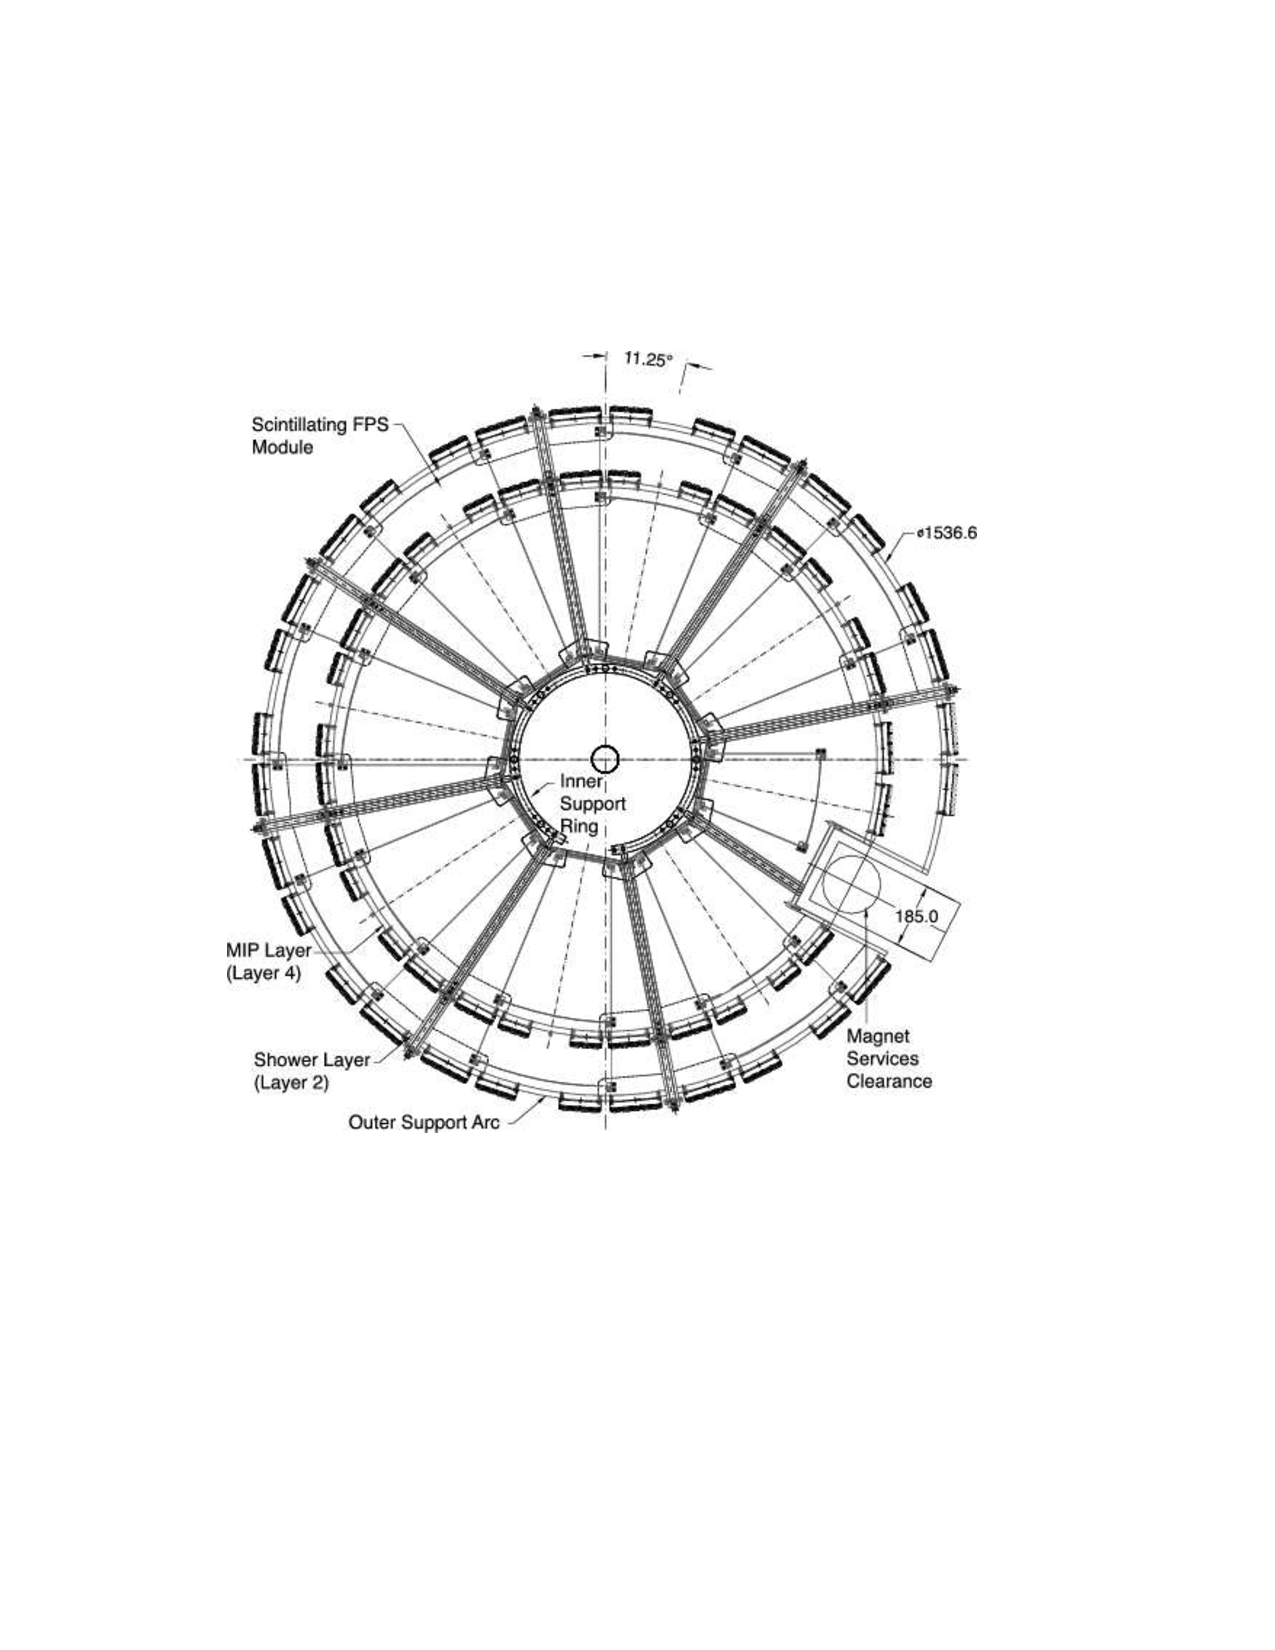
\includegraphics[height=0.5\textheight, width=0.5\textwidth]{./Images/29_PS_forward_01.pdf}
      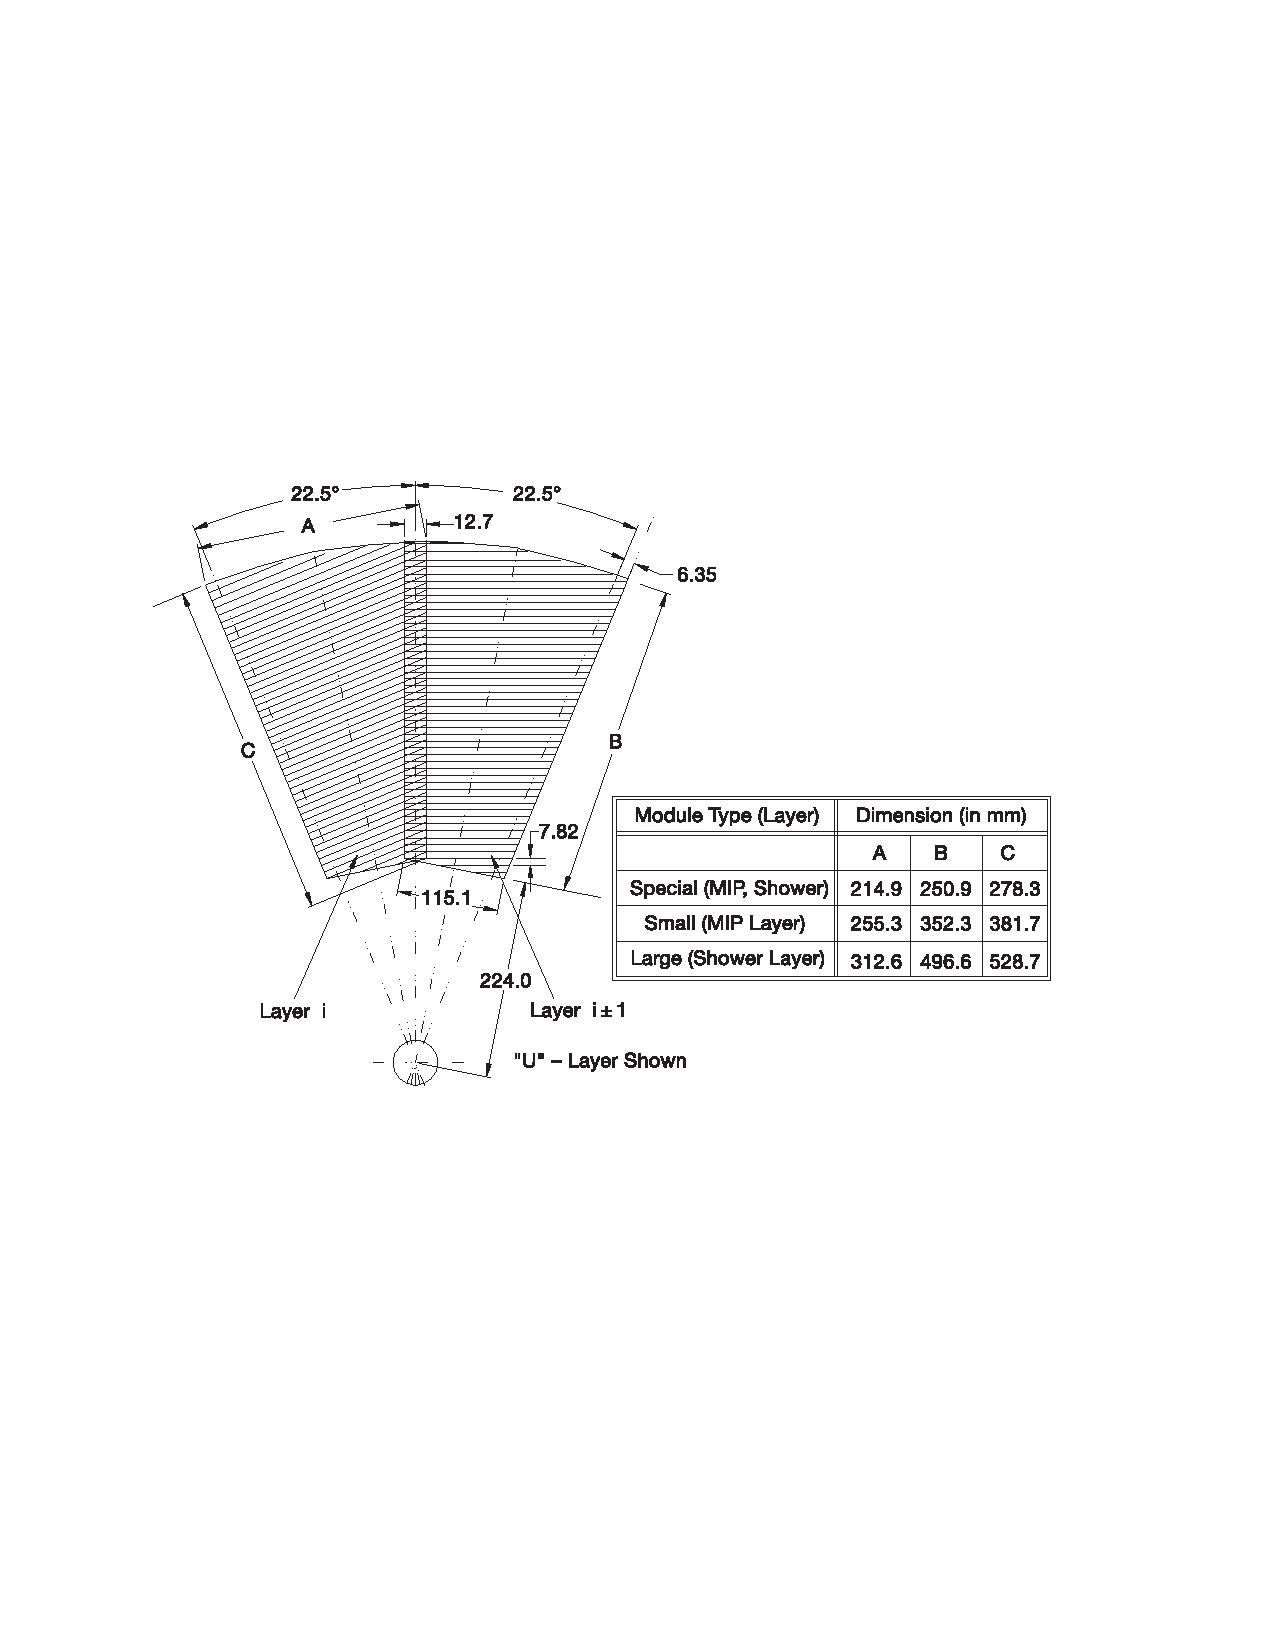
\includegraphics[height=0.5\textheight,width=0.5\textwidth]{./Images/29_PS_forward_modules.pdf}
      \caption*{$r-\phi$ view of the north FPS detector. For clarity,
        only layers 2 (shower) and 4 (MIP) are shown; layers 1
        (shower) and 3 (MIP) are rotated by 22.5 degrees in $\phi$ with respect to
        these layers so their supports do not overlap.}
    \end{figure} 
\end{overlayarea}
\end{frame}


%%%%%% SLIDE
\begin{frame}{\textcolor{Goldenrod}{Forward Preshower Detector}}
  \begin{overlayarea}{\textwidth}{\textheight}
    \begin{figure}[h]\centering
      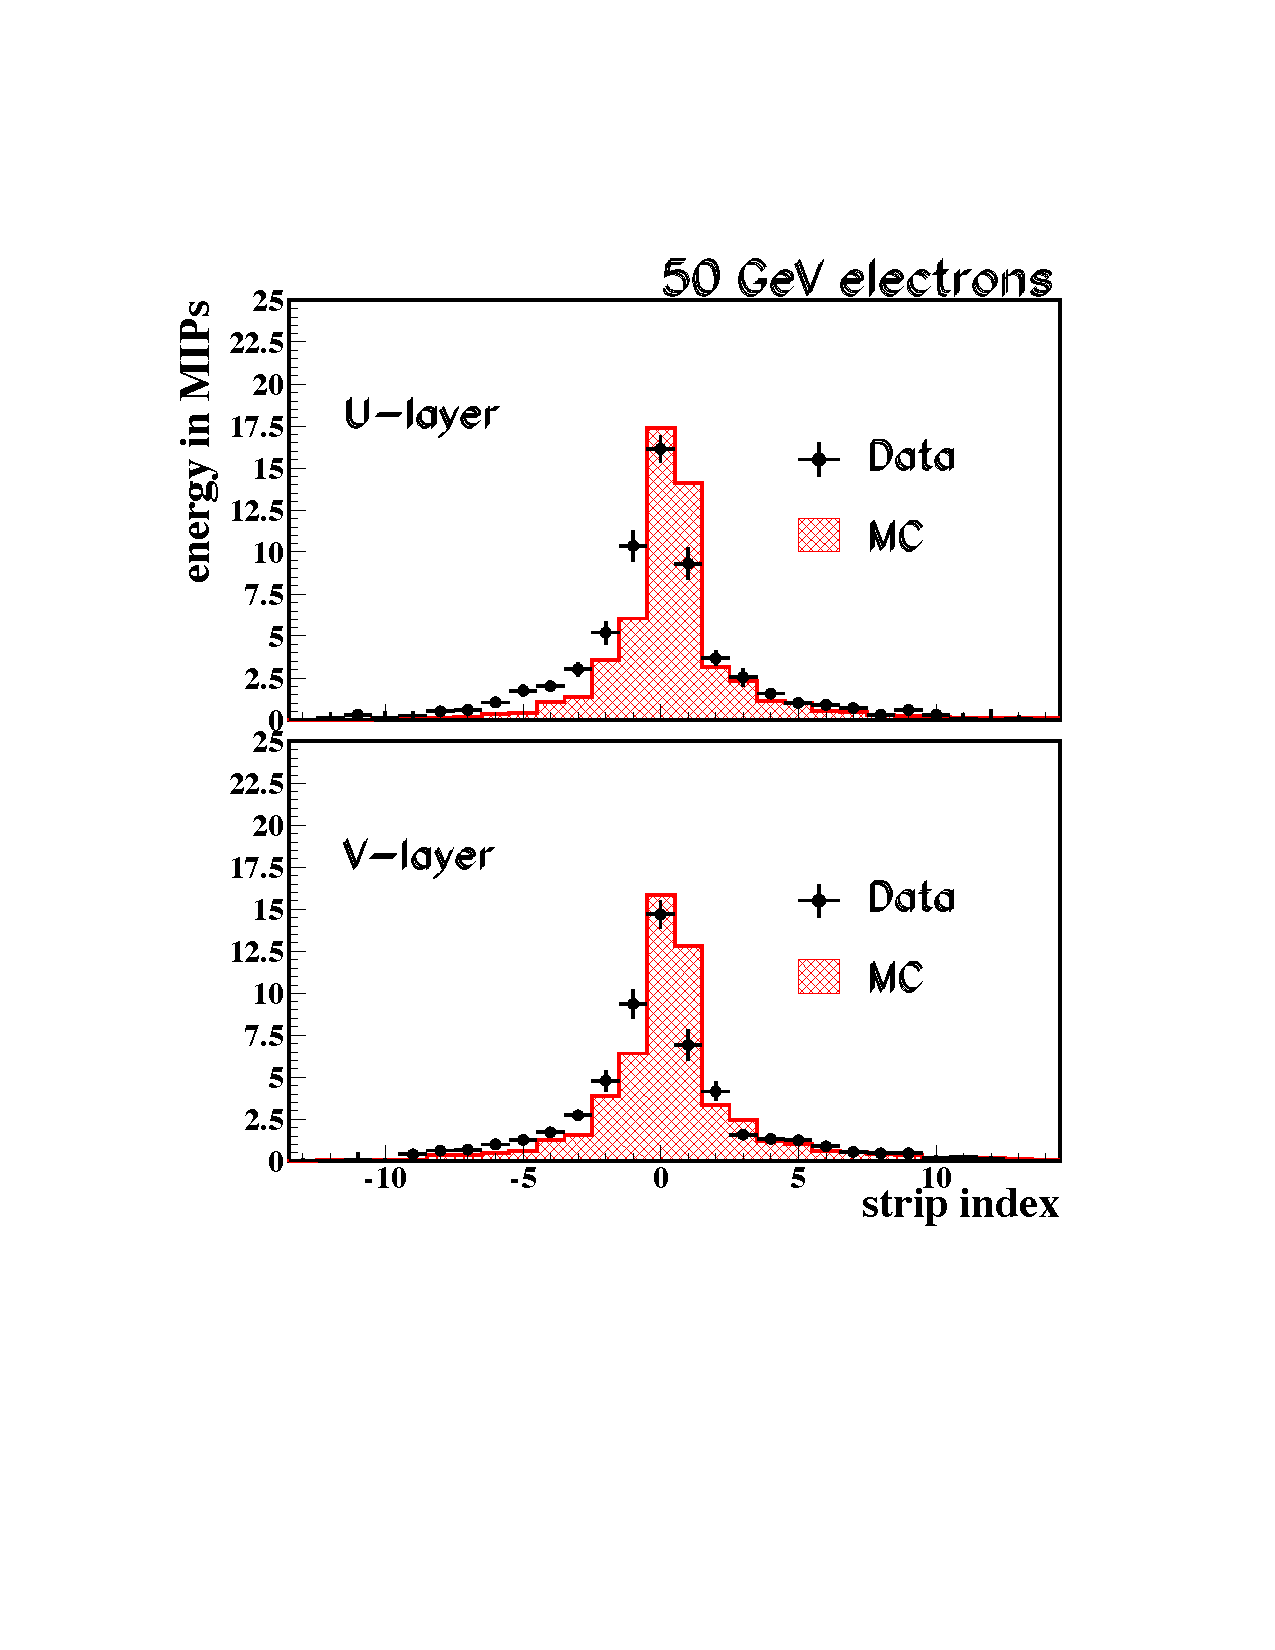
\includegraphics[height=0.45\textheight, width=0.5\textwidth]{./Images/29_PS_performance.pdf}
      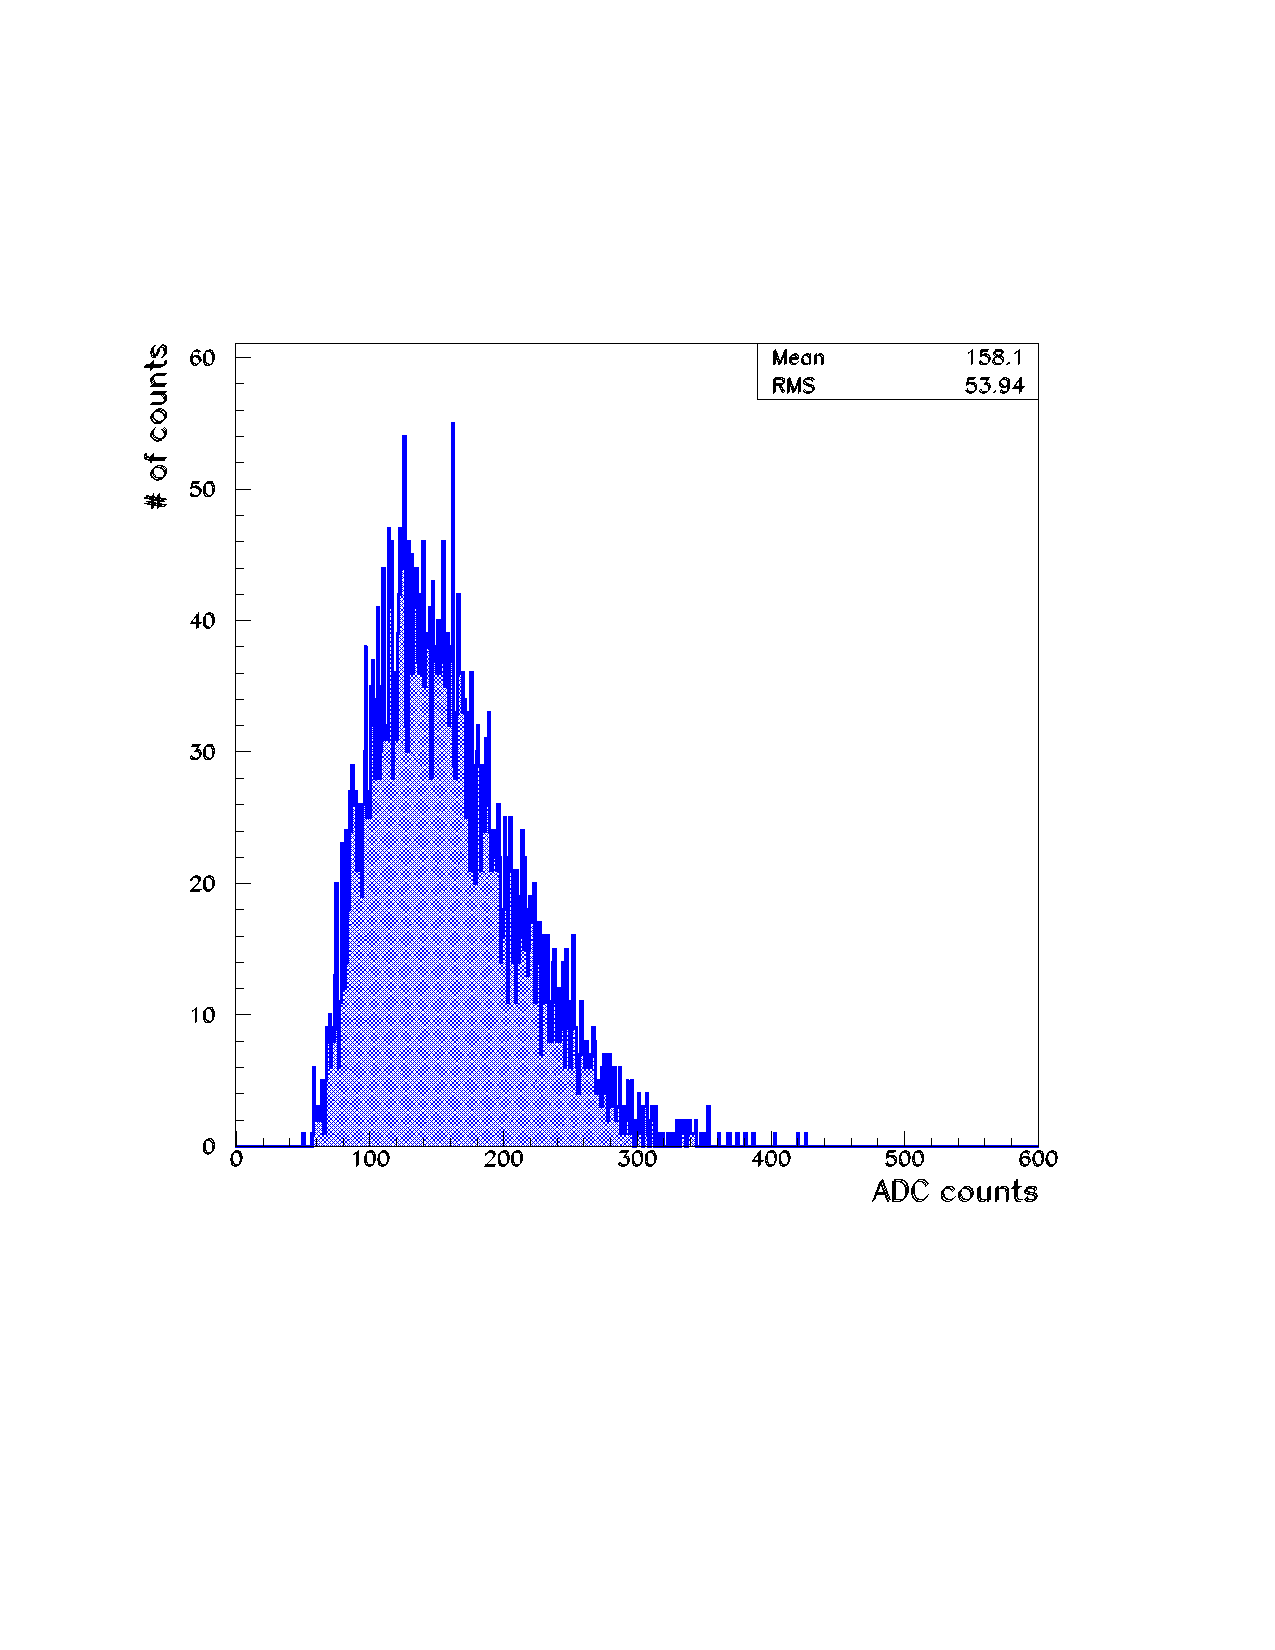
\includegraphics[height=0.45\textheight,width=0.5\textwidth]{./Images/29_PS_performance_01.pdf}
      
    \end{figure} 
    \itt
  \item left: the shower
    profile of $50 GeV$ electrons in the FPS for both the u and the v
    module layers.
  \item right:
    The MIP spectrum for $125$ GeV pions traversing the u layer of
    the forward FPS module.
    \note{The spectrum is an event by event sum
      of the two adjacent hit strips}
    \tti
\end{overlayarea}
\end{frame}
